\RequirePackage[l2tabu, orthodox]{nag}
\documentclass[10pt]{scrartcl}
% \documentclass[10pt]{article}
\usepackage[T1]{fontenc}
\usepackage{amsmath,amsfonts,amssymb}
\usepackage{mathtools}
\usepackage{color,soul}
\usepackage{fullpage}
\usepackage{enumerate}
\usepackage{graphicx}
\usepackage[colorlinks=true,urlcolor=blue]{hyperref}
\usepackage{cleveref} % MUST BE AFTER HYPERREF
\usepackage{floatrow}
\usepackage{deluxetable}
\usepackage{verbatim}
\usepackage{fancyvrb}
\usepackage{listings}
\usepackage[activate={true,nocompatibility},final,tracking=true,kerning=true,spacing=true,factor=1100,stretch=10,shrink=10]{microtype}
\usepackage{calc}
\usepackage[font=small]{caption}
\usepackage[font=scriptsize]{subcaption}

\floatsetup{ 
  heightadjust=object,
  valign=t
}

\definecolor{Light}{gray}{.90}
\sethlcolor{Light}

\lstset{%
language=IDL,                   % choose the language of the code
basicstyle=\footnotesize\sffamily,%\ttfamily\footnotesize,       % the size of the fonts that are used for the code
numbers=left,                   % where to put the line-numbers
numberstyle=\footnotesize,      % the size of the fonts that are used for the line-numbers
stepnumber=1,                   % the step between two line-numbers. If it is 1 each line will be numbered
numbersep=5pt,                  % how far the line-numbers are from the code
showspaces=false,               % show spaces adding particular underscores
showstringspaces=false,         % underline spaces within strings
showtabs=false,                 % show tabs within strings adding particular underscores
% frame=single,                   % adds a frame around the code
backgroundcolor=\color{Light},
columns=flexible,
tabsize=2,                      % sets default tabsize to 2 spaces
captionpos=b,                   % sets the caption-position to bottom
breaklines=true,                % sets automatic line breaking
breakatwhitespace=false,        % sets if automatic breaks should only happen at whitespace
escapeinside={\%*}{*)}          % if you want to add a comment within your code
}

\title{Code Explanation}
\author{Jeren Suzuki}
\date{Last Edited \today}

\begin{document}

\maketitle
\pagenumbering{Roman}
\tableofcontents
\addcontentsline{toc}{section}{Introduction}
\clearpage
\pagenumbering{arabic}

\section*{Introduction} % (fold)
\label{sec:introduction}
This pdf is meant to illustrate what each step of the code is doing. The code is split up into four major parts. Preparing parameters, thresholding image to find suns, limb-fitting whole suns, and finding fiducials. 
% section introduction (end)

\section{Preparing Parameters} % (fold)
\label{sec:preparing_parameters}

\subsection{Loading Image} % (fold)
\label{sub:loading_image}
This is the starting image we use to analyze for sun centering and fiducial finding.
\begin{figure}[!ht]
    \centering
    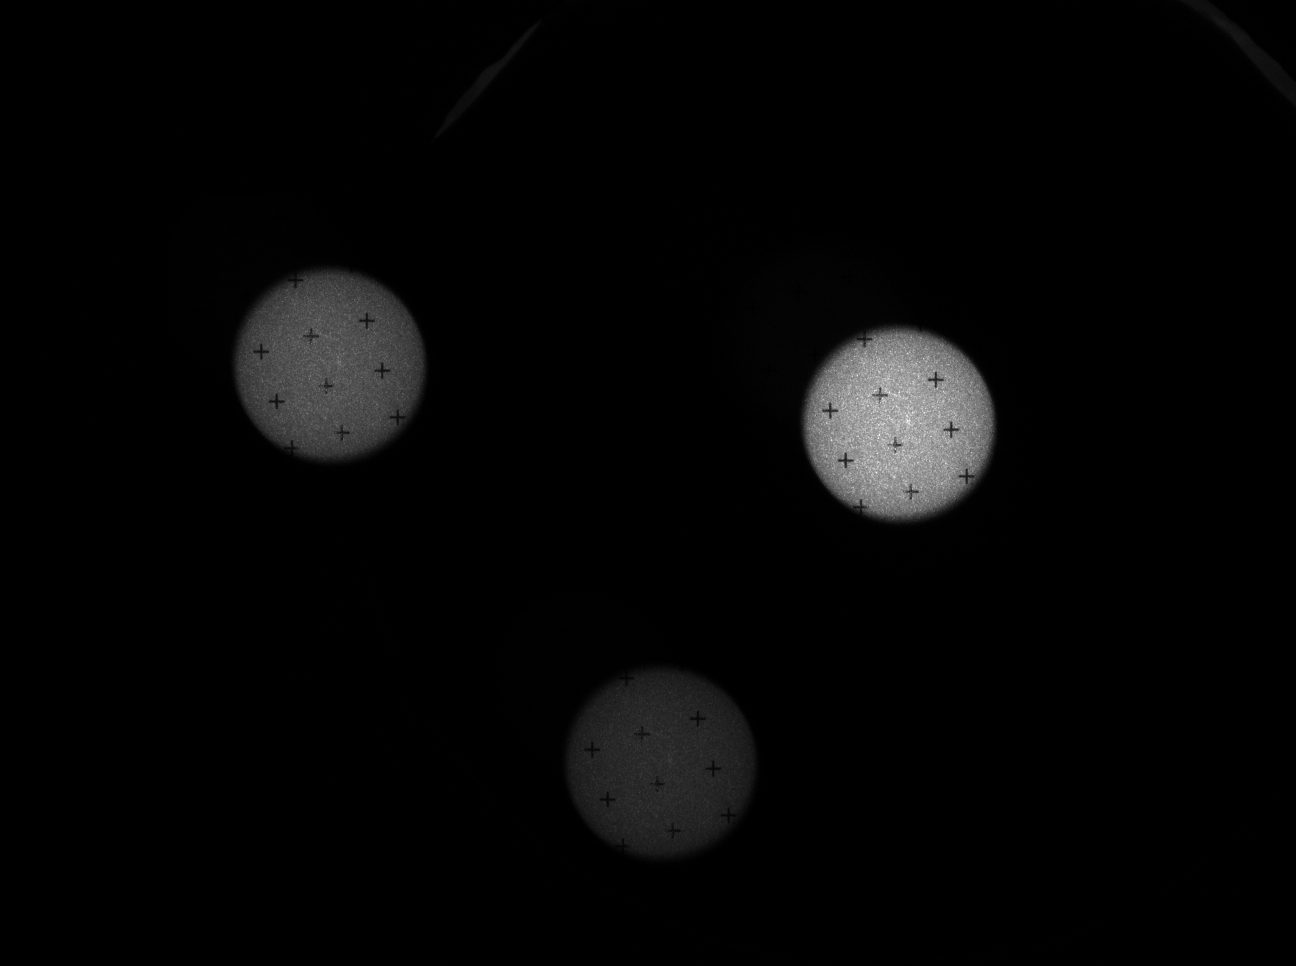
\includegraphics[width=.9\textwidth]{../plots_tables_images/tritest.jpg}    
    \caption{}
    \label{flowchart}
\end{figure}

% subsection loading_image (end)

\newpage

\subsection{Reading In Parameter Block} % (fold)
\label{sub:reading_in_parameter_block}

\begin{lstlisting}
scan_width 10               ; Distance to next chord when picking chords to limb-fit
sundiam 70                  ; Approx Solar diameter, deprecated
nstrips 5                   ; Number of pairs of solar chords to limb-fit per direction
ministrip_length 4          ; Length of limb profile to linear fit
crop_box 120                ; Half-width of box used to find fiducials in
elim_perc 1                 ; Percentage of highest pixels to eliminate when finding threshold
n_smooth 900                ; Elements to smooth by when finding threshold 
border_pad 50               ; If solar center is within this value of border, marked as a partial sun
triangle_size .25           ; Percentage of image height to use for triangle sides for making clipped-bottom-corner mask
fid_smooth_thresh -150      ; Threshold to determine row/column positions of fiducials
onedsumthresh 80            ; Once looking at fiducial candidates, look at 1D sum of smaller fiducial crop and threshold difference of smoothed array - original array by this
disk_brightness 15          ; Arbitrary pixel brightness to eliminate bright fiducial candidates which are on the solar disk but are not on a fiducial
fid_crop_box 15             ; Half-width of box used to analyze fiducials
fid_smooth_candidates 15    ; Smoothing paramater for 1D sums of fiducial candidates 

\end{lstlisting}
% subsection reading_in_parameter_block (end)                 
% section preparing_parameters (end)

\section{Thresholding Image} % (fold)
\label{sec:thresholding_image}

After we read in the necessary parameters, we turn our attention to thresholding the image to find the centers of the suns. Starting with the initial image, we sort the image according to pixel values and see a grouping of differently dimmed suns. 

\begin{figure}[!ht]
    \centering
    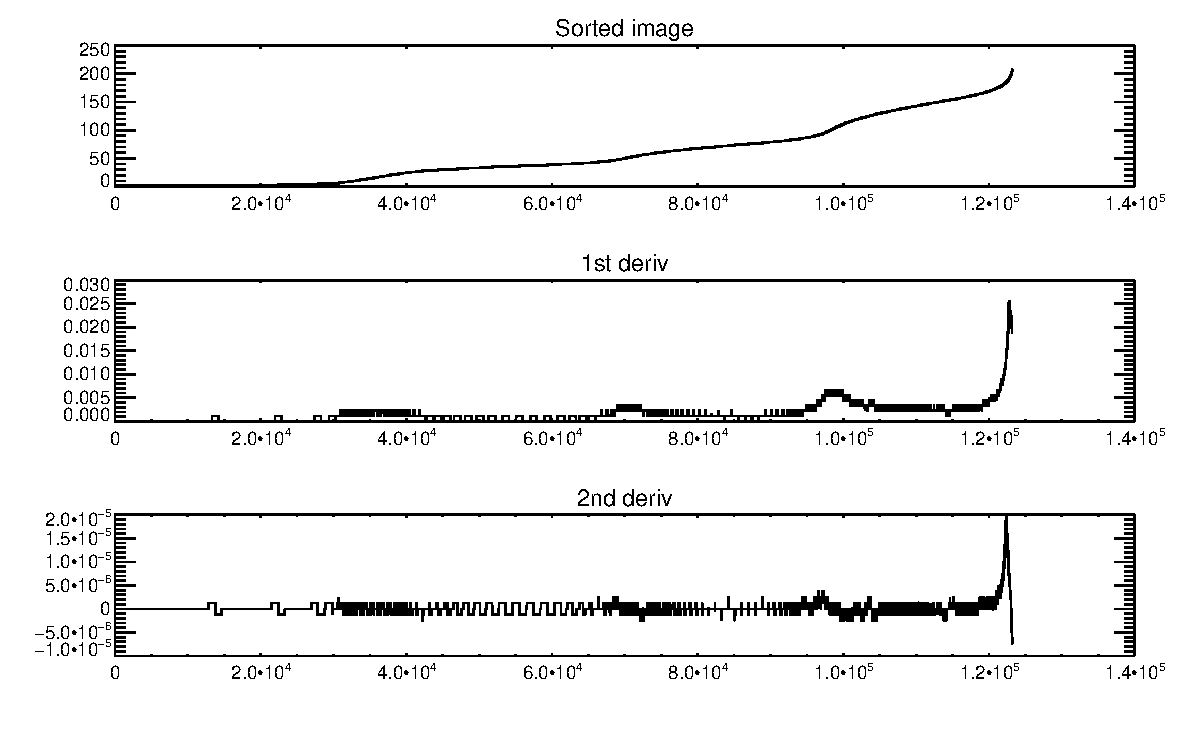
\includegraphics[width=.9\textwidth]{../plots_tables_images/sortedarray.eps}    
    \caption{We look at the second derivative because it consistently quantifies the thresholds to identify each solar region by. With the right-most part of the 2nd derivative zeroed out, we identify the three peaks corresponding to what pixel value we should threshold by to separately identify each sun.}
    \label{sortedarray}
\end{figure}

Using these three thresholds, we create separate masks, one for each sun. 

\begin{figure}[!ht]
\ffigbox{
    \begin{subfloatrow}
        \ffigbox[.6\FBwidth]% Width of subfloat
        {
        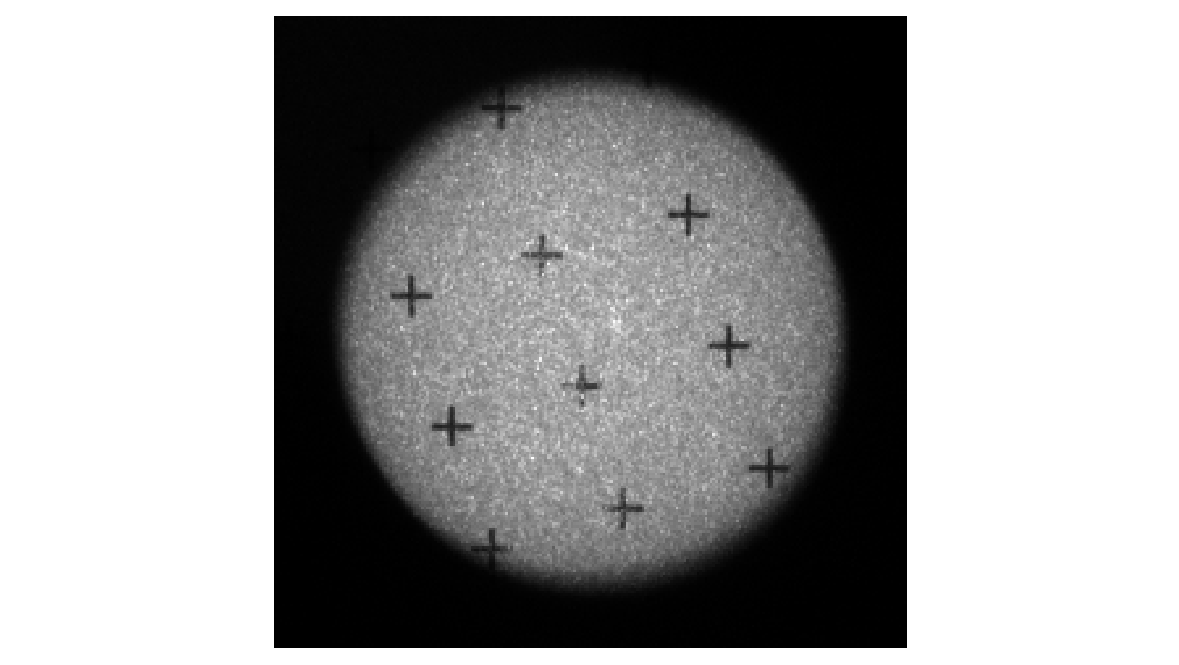
\includegraphics[width=\linewidth]{../plots_tables_images/tritest_reg1}
        }
        {
        \subcaption{100\% brightness region, henceforth Region 1}
        }
    \end{subfloatrow}
    \begin{subfloatrow}
        \ffigbox[.6\FBwidth]% Width of subfloat
        {
        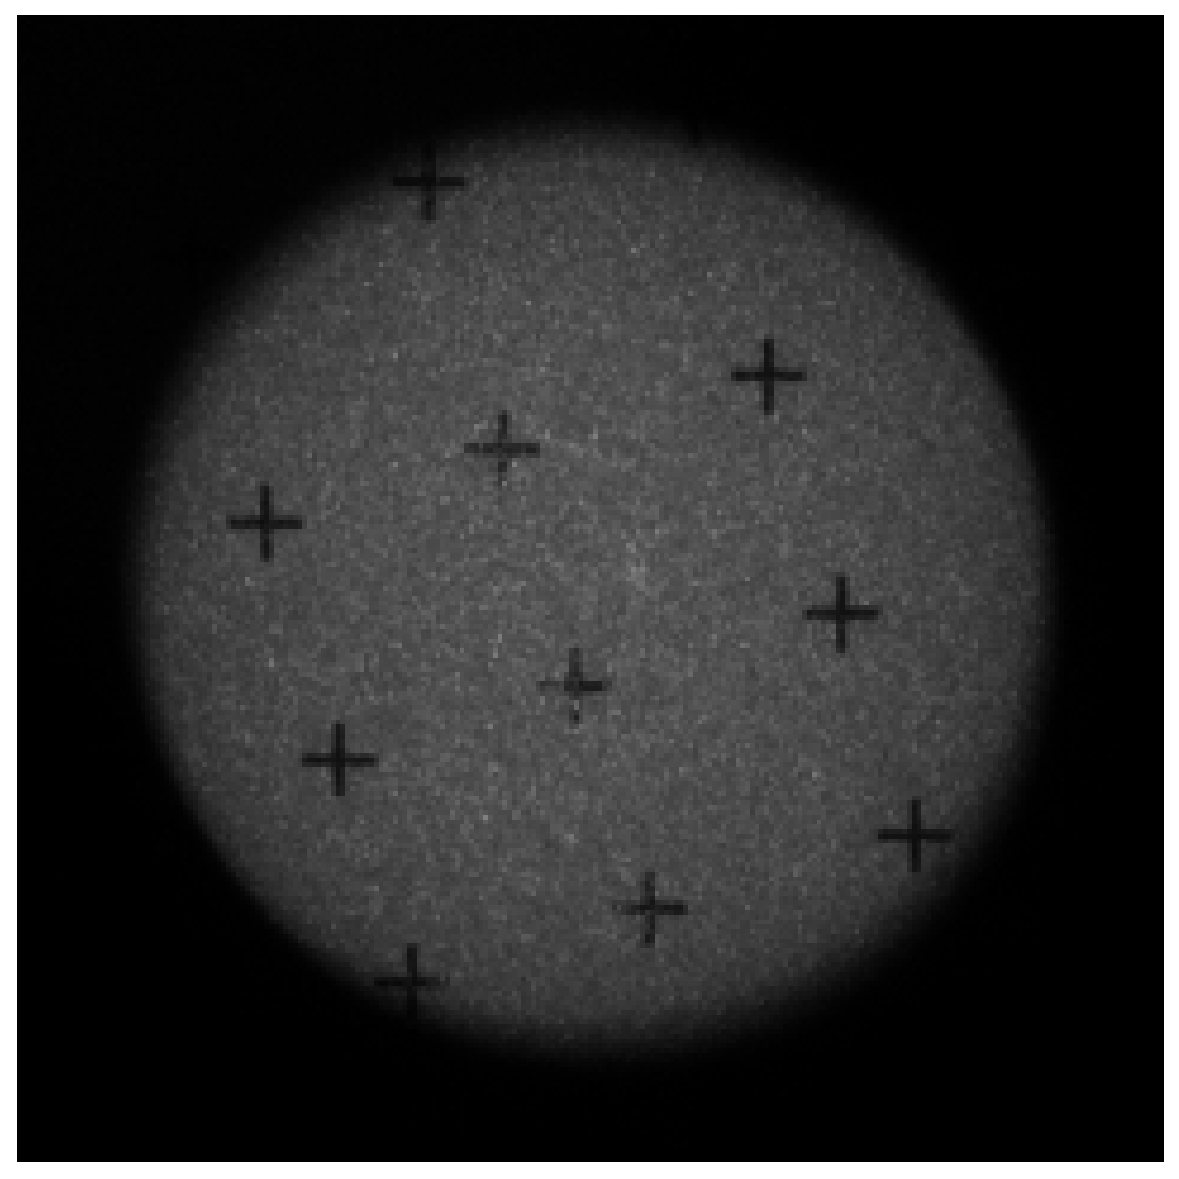
\includegraphics[width=\linewidth]{../plots_tables_images/tritest_reg2}
        }
        {
        \subcaption{50\% brightness region, henceforth Region 2}
        }
    \end{subfloatrow}
        \begin{subfloatrow}
        \ffigbox[.6\FBwidth]% Width of subfloat
        {
        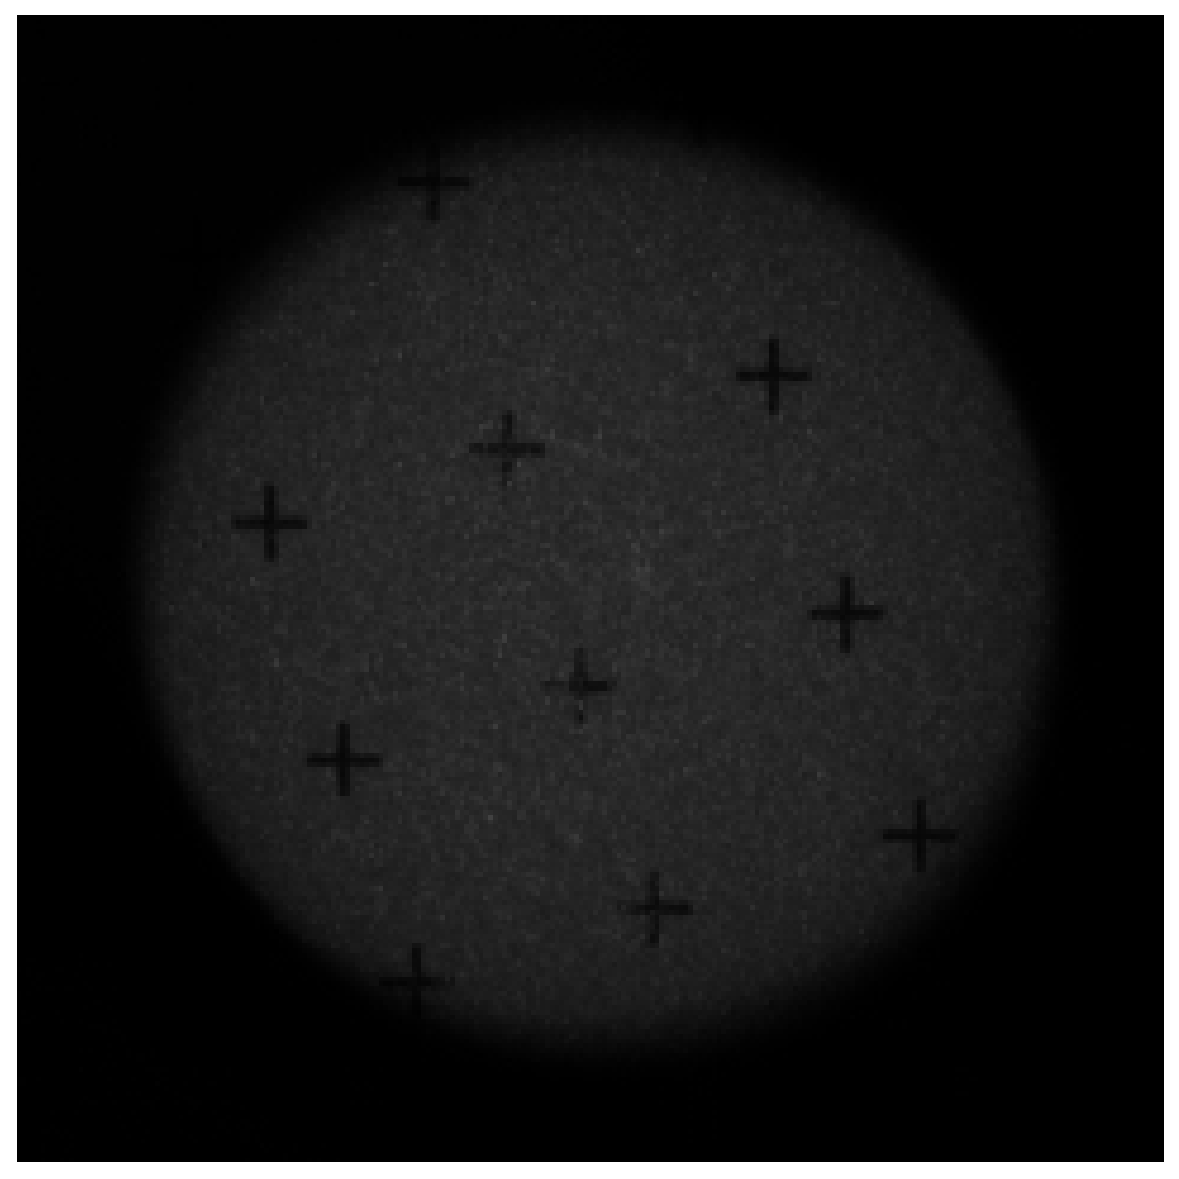
\includegraphics[width=\linewidth]{../plots_tables_images/tritest_reg3}
        }
        {
        \subcaption{25\% brightness region, henceforth Region 3}
        }
    \end{subfloatrow}
}
{\caption{}
\label{triplecrop}}
\end{figure}

% section thresholding_image (end)

\subsection{Quick mask centering} % (fold)
\label{sub:quick_mask_centering}

	Now that we have three cropped regions, we have to identify what brightnesses they are. We do this by looking at a low enough threshold that all the solar pixels for every brightness are included in the mask but not any of the background pixels. We then use IDL's \hl{\texttt{LABEL\_REGION}} to assign a label number to each shape. A shape is defined to be a mask where there are adjacent pixels. If done correctly, we end up with 3 shapes that have now had their values replaced with what index they have been assigned. For this image, we have three regions, one a mask of 1s, one a mask of 2s, and one of 3s. Now we use \hl{\texttt{HISTOGRAM}} to bin these shapes and thus their locations. For each mask, we calculate the average value of the pixels from the starting image and  






	We find the centers of each cropped region in \cref{triplecrop} using a simple masking method. With the centroid determined by a simple masking method, we have to make sure that the center is from a whole sun. The process so far has not taken into account any spatial information so the next step is to look at a border region of the mask. 

% \begin{figure}[!ht]
% \ffigbox{
%     \begin{subfloatrow}
%         \ffigbox[\FBwidth]% Width of subfloat
%         {
%         
\includegraphics[width=.9\linewidth]{../plots_tables_images/cutcorner.eps}
%         }
%         {
%         \subcaption{What our mask should look like - side of black triangle is 1/4 of image width}
%         \label{noborder}
%         }
%     \end{subfloatrow}
%     \begin{subfloatrow}
%         \ffigbox[\FBwidth]% Width of subfloat
%         {
%         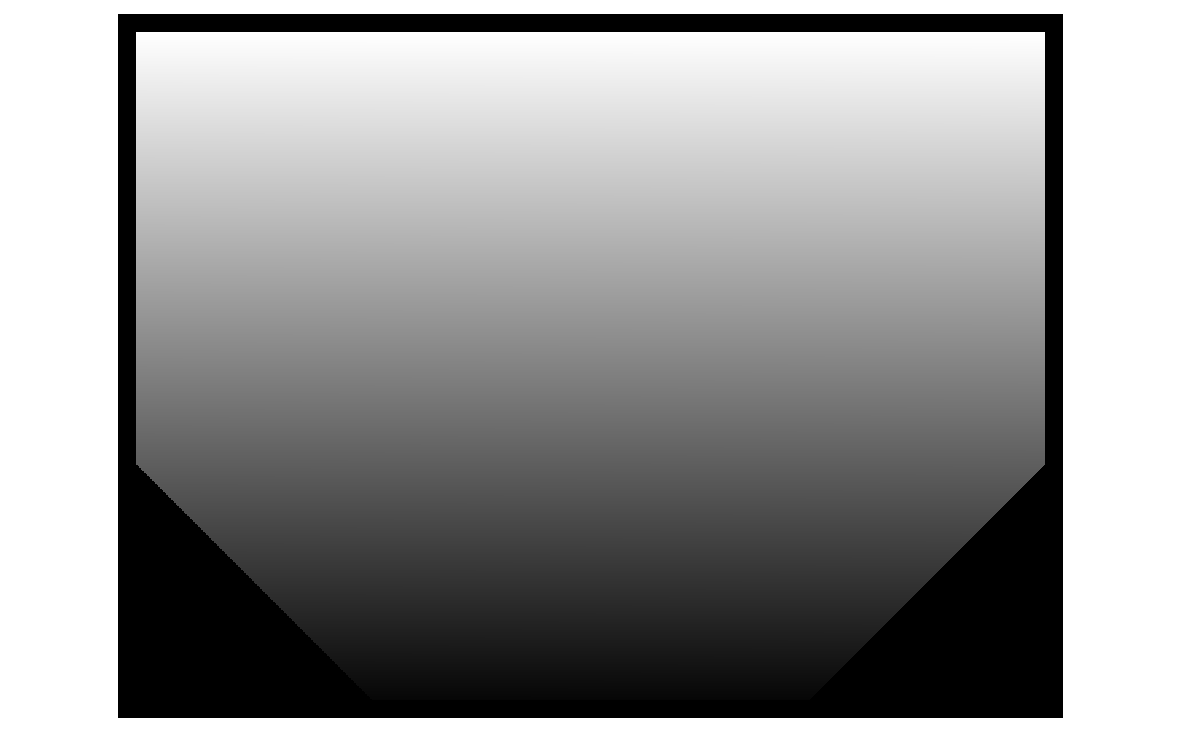
\includegraphics[width=.9\linewidth]{../plots_tables_images/cutcornerwborder.eps}
%         }
%         {
%         \subcaption{A proposed mask that looks within a certain distance form the border.}
%         \label{aborder}
%         }
%     \end{subfloatrow}
% }
% {\caption{The bottom corners will never see any data; the border mask takes into account the distance from the hypotenuse of the bottom corners}
% \label{cuttingcorners}
% }
% \end{figure}


% If the center we computed with the mask method is within a certain distance to the edge of the image (as shown in Figure \ref{aborder}), we mark that solar region as ``\emph{partial}'' and cease further analysis for that particular brightness sun. \\
% \indent Once we have our list of whole suns along with their masked centers, we proceed to fitting the solar limbs to find a more accurate center.


\begin{figure}[!ht]
    \centering
    
\includegraphics[width=.9\textwidth]{../plots_tables_images/cutcorner.eps}    
    \caption{What our mask should look like - side of black triangle is 1/4 of image width}
    \label{dogeared}
\end{figure}

To check if the sun is a partial sun, we calculate the distance of the measured center to the edges of the image. If the center of the sun is too close to the edge, then there must be a part of the sun that is cut off in the image. This method works simply for a rectangular mask but our mask is not so simple. The bottom corners of our mask are cut off, essentially making it so that that part of the mask will never see any rays of light. See \cref{dogeared}. To deal with the distance from the edges of the bottom corners, we rotate the coordinates of the center by 45 degrees. 

\begin{figure}[!ht]
\ffigbox{
    \begin{subfloatrow}
        \ffigbox[\FBwidth]% Width of subfloat
        {
        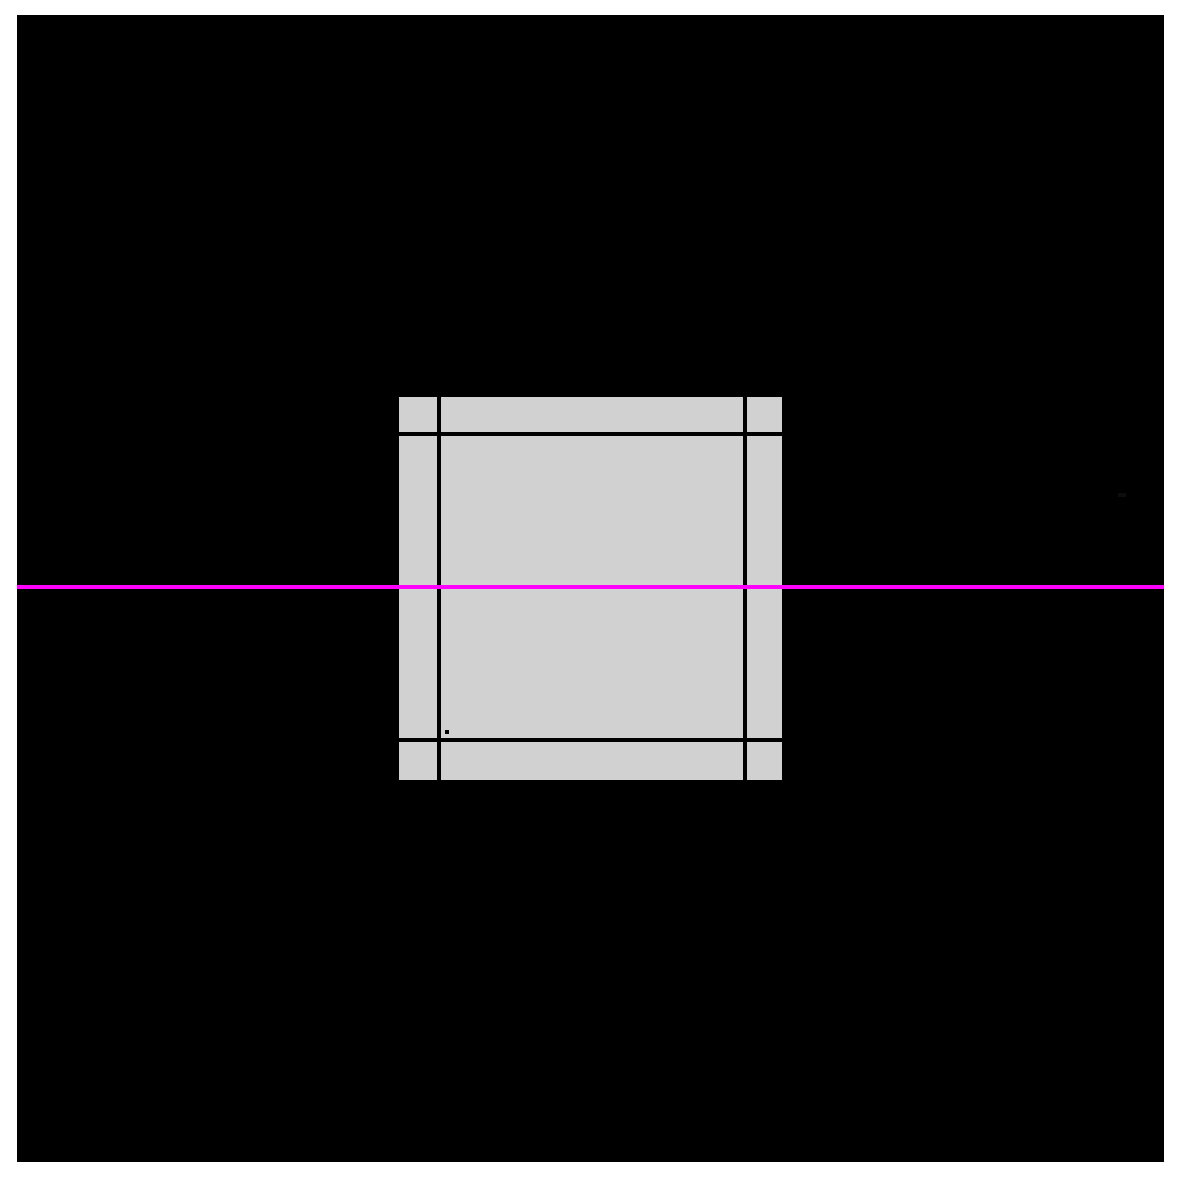
\includegraphics[width=.9\linewidth]{../plots_tables_images/firstcheck.eps}
        }
        {
        \subcaption{The black lines represent 10\% of the width/height and the hypothetical solar center is the black dot in the lower lefthand corner. As you can see, by this simple check's standards, the center is OK (but it's actually in the corner which is bad).}
        \label{noborder}
        }
    \end{subfloatrow}
    \begin{subfloatrow}
        \ffigbox[\FBwidth]% Width of subfloat
        {
        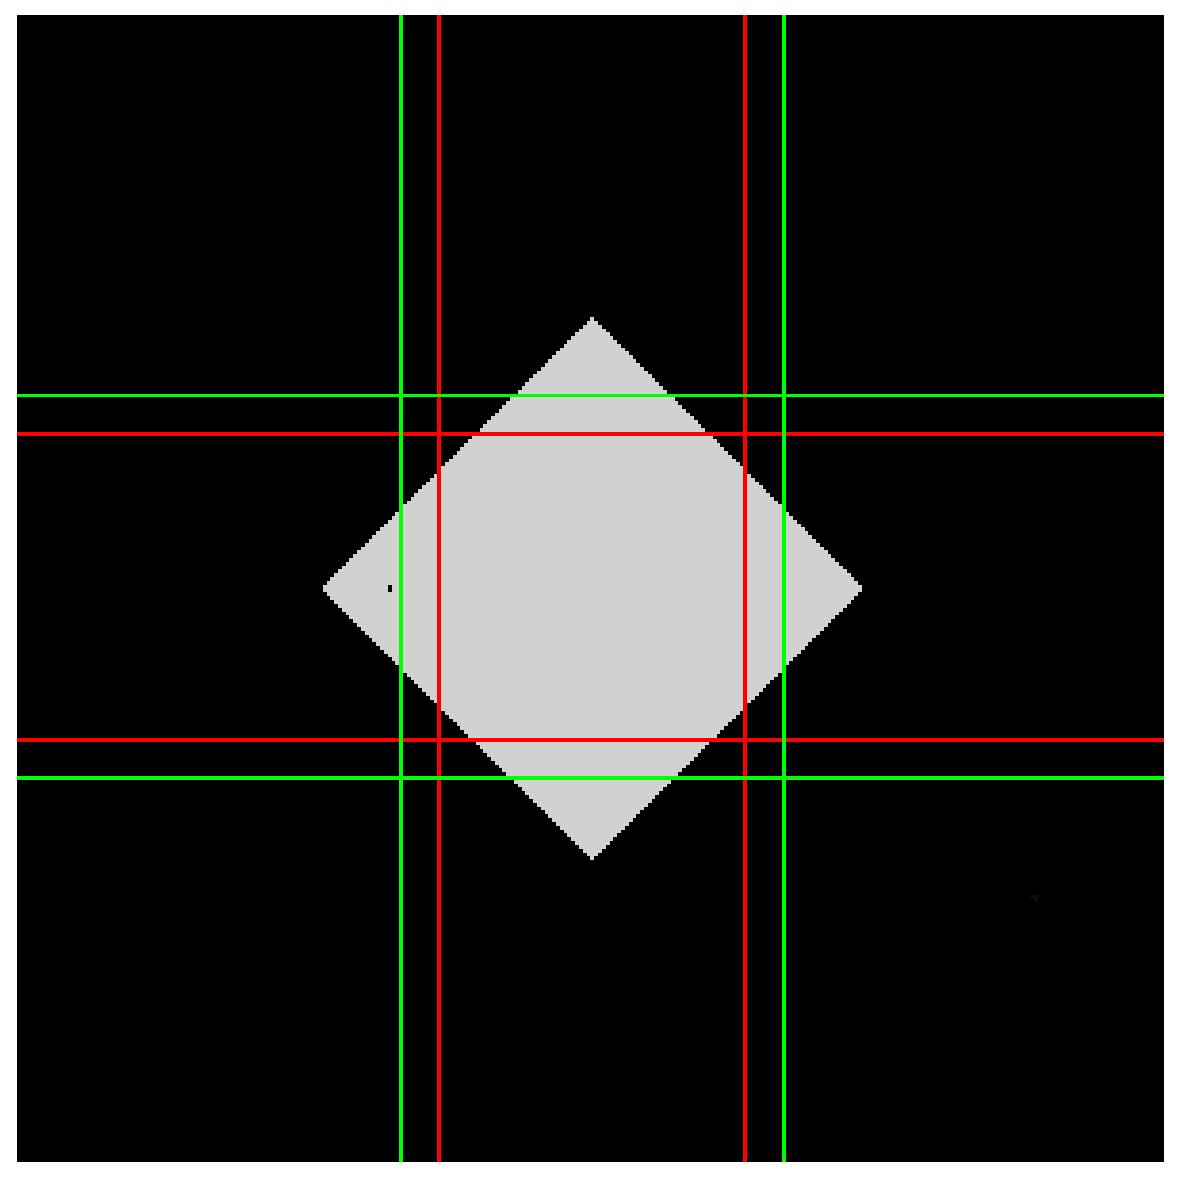
\includegraphics[width=.9\linewidth]{../plots_tables_images/seccheck.eps}
        }
        {
        \subcaption{The green lines outline the shape of the box in \cref{noborder} while the red lines outline the shape of the box 10\% from the edges. By rotating the black dot (or in this case, the gray square) and checking if it is within 10\% of the edge, we can essentially check the distance from the diagonal corner borders.}
        \label{aborder}
        }
    \end{subfloatrow}
}
{\caption{By combining two edge checks, one with 45$^\circ$ rotated coordinates, we can quickly calculate the distance from the edge of the mask.}
\label{cuttingcorners}
}
\end{figure}
% subsection quick_mask_centering (end)

\section{Limb Fitting} % (fold)
\label{sec:limb_fitting}

We cut 5 chords centered around the masked center position in both axes (See \cref{chords}). With the same threshold found in \cref{sec:thresholding_image}, we look at where the chord profile crosses the threshold (See \cref{limbs}). We use a four-pixel limb profile with 2 pixels above the threshold and 2 pixels below the threshold. We then do a linear fit on these four pixels to see where it crosses the threshold. With a pair of limb-fitted threshold crossing points, we create a chord and find it's center. Doing this 5 times, we average the positions of the chord centers to be the limb-fitted center position. 

\begin{figure}[!ht]
\ffigbox{
    \begin{subfloatrow}
        \ffigbox[\FBwidth-2.0cm]% Width of subfloat
        {
        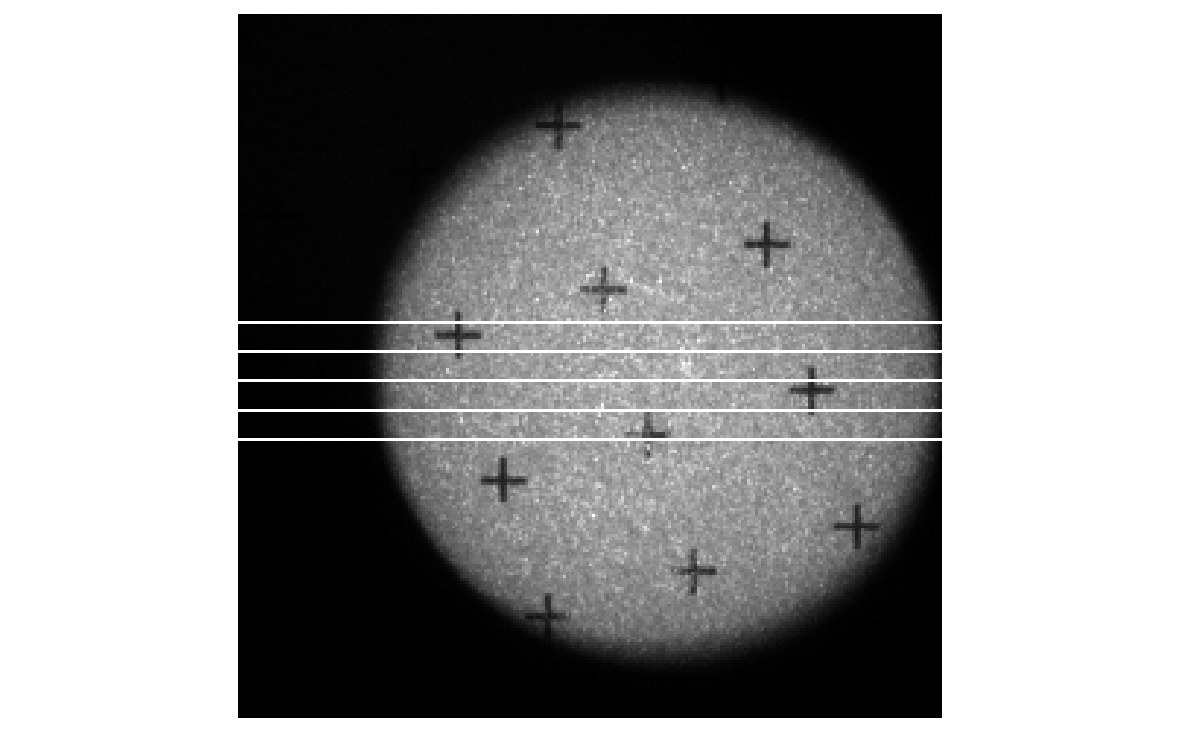
\includegraphics[width=.9\linewidth]{../plots_tables_images/5chords.eps}
        }
        {
        \subcaption{The middle chord passes through the center of the sun}
        \label{chords}
        }
    \end{subfloatrow}
    \begin{subfloatrow}
        \ffigbox[\FBwidth+2.0cm]% Width of subfloat
        {
        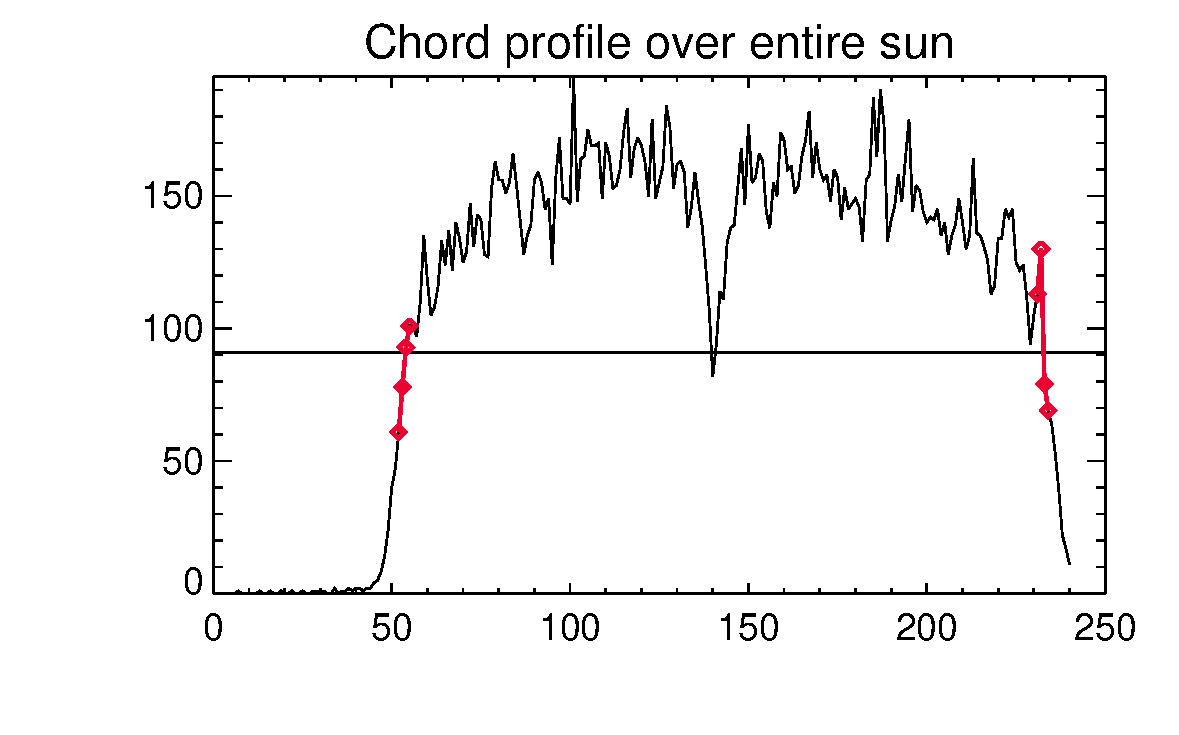
\includegraphics[width=.9\linewidth]{../plots_tables_images/redlimbs.eps}
        }
        {
        \subcaption{The indices in red are the pixels we apply a linear fit to see where it crosses the threshold (which is the horizontal line).}
        \label{limbs}
        }
    \end{subfloatrow}
}
{\caption{}
\label{sup}}
\end{figure}

% section limb_fitting (end)

\section{Finding Fiduials} % (fold)
\label{sec:finding_fiduials}

Now with limb-fitted centers, we re-crop the image to work with (It shouldn't look much different than \cref{triplecrop} if we masked the centers correctly).

\subsection{First 1D Sum} % (fold)
\label{sub:first_1d_sum}

To find fiducials, we calculate a 1D sum in one direction and look for dips in the array corresponding to fiducials. 

\begin{figure}[!ht]
\ffigbox{
    \begin{subfloatrow}
        \ffigbox[\FBwidth]% Width of subfloat
        {
        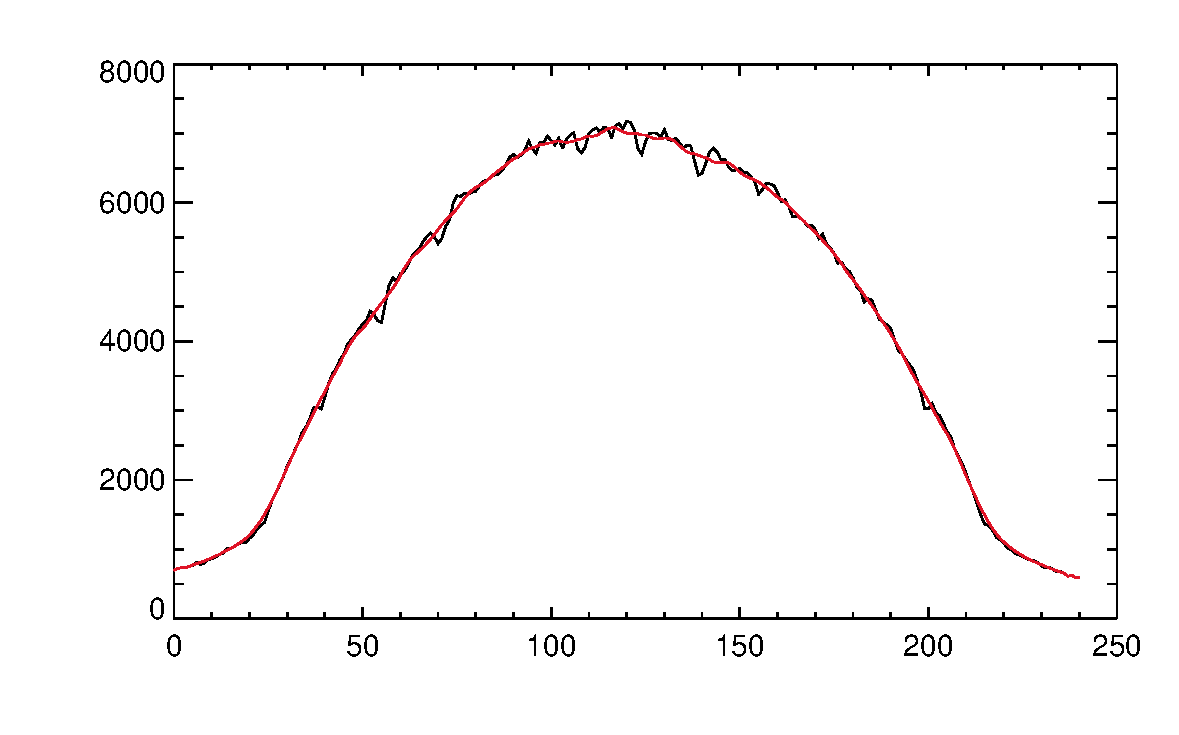
\includegraphics[width=.9\linewidth]{../plots_tables_images/smooth_expl.eps}
        }
        {
        \subcaption{This is the 1D sum of a solar image. The line in red is the sum smoothed by 10 pixels.}
        \label{doublelines}
        }
    \end{subfloatrow}
    \begin{subfloatrow}
        \ffigbox[\FBwidth]% Width of subfloat
        {
        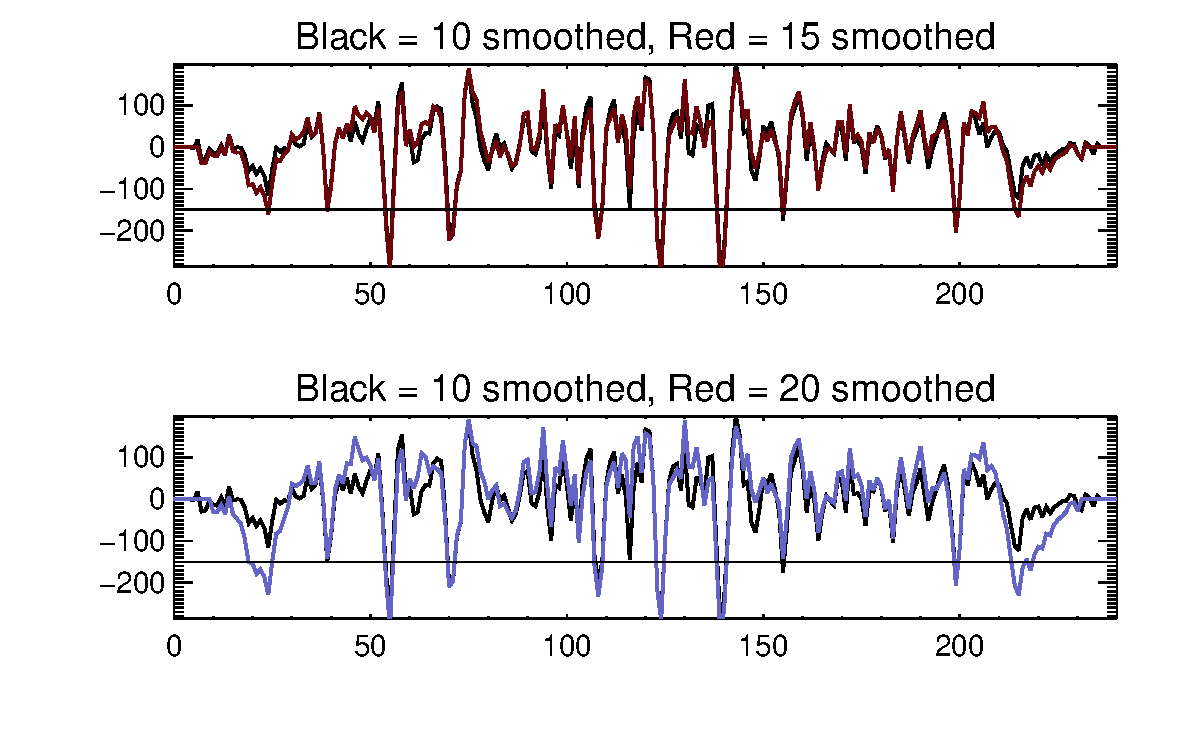
\includegraphics[width=.9\linewidth]{../plots_tables_images/smoothcomp.eps}
        }
        {
        \subcaption{We subtract the smoothed profile from the raw data to emphasize dips. Comparisons of the smooth amount change the width and number of the dips, although not really the depth. It says ``Red'' in the title, but it's really blue. Typo.}
        \label{threshed}
        }   
    \end{subfloatrow}
}
{
\caption{}
\label{smoothed}
}
\end{figure}

After thresholding the difference of the 1D sum from it's smoothed counterpart, we identify the column/row positions of fiducials. 
% subsection first_1d_sum (end)

\subsection{Ruling Out False Fiducial} % (fold)
\label{sub:ruling_out_false_fiducial}

With a bunch of x and y locations of fiducials, we have to determine which pairs of coordinates are actually fiducials. The first step is to look at each possible pair and eliminate those that are too bright. This affects candidates which are located on the solar disk but do not lie on fiducials. See \cref{rulingout}.


\begin{figure}[!ht]
\ffigbox{
    \begin{subfloatrow}
        \ffigbox[\FBwidth]% Width of subfloat
        {
        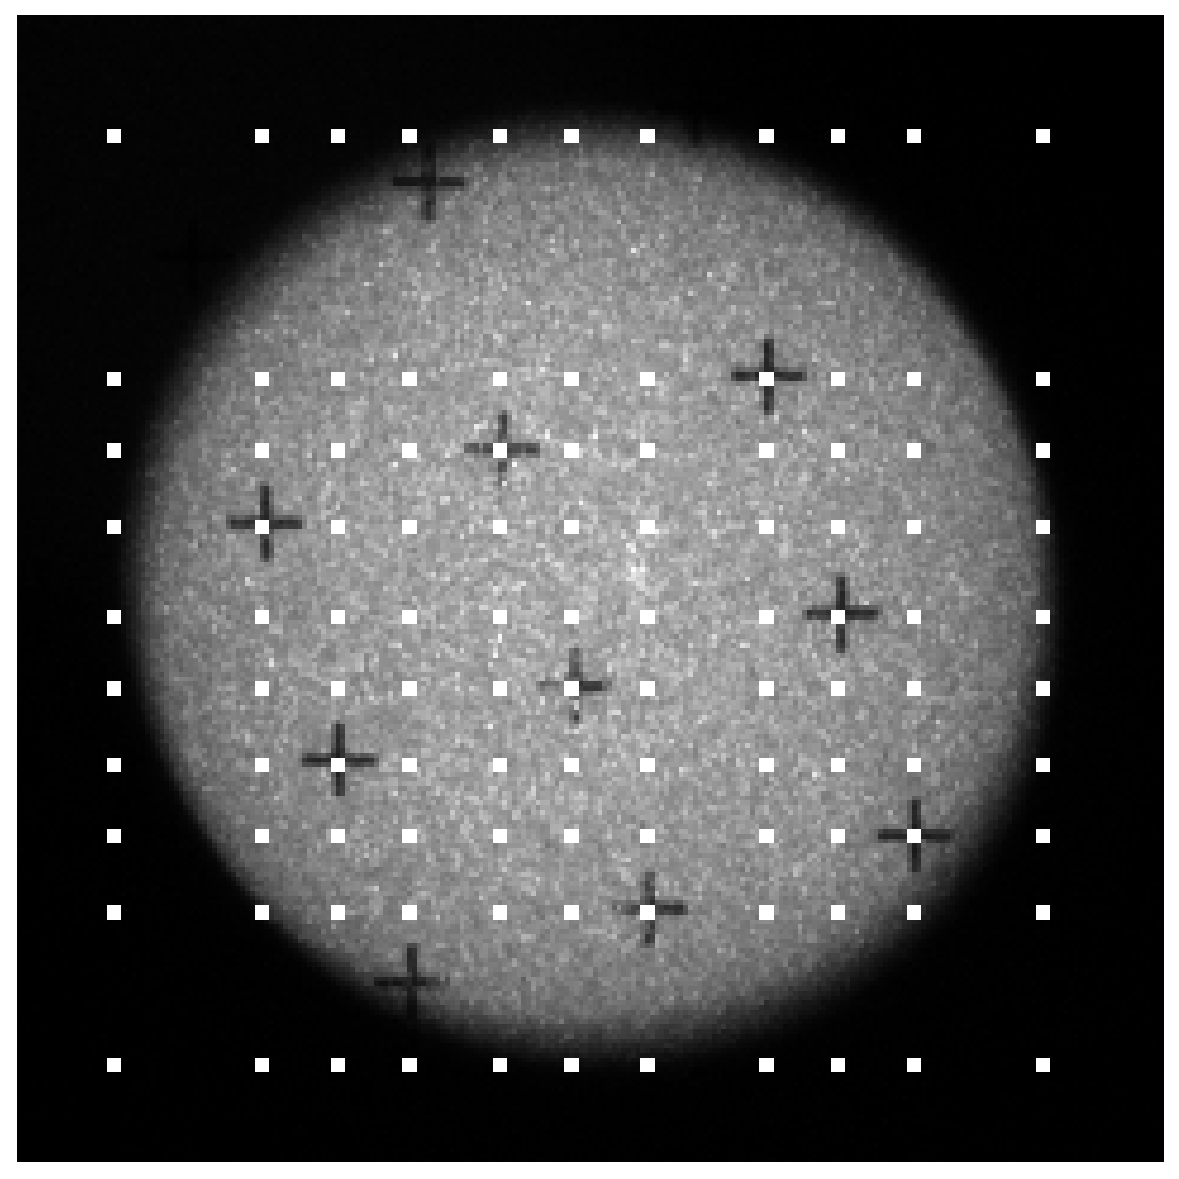
\includegraphics[width=.9\linewidth]{../plots_tables_images/allfid.eps}
        }
        {
        \subcaption{All possible positions of fiducials according to first 1D sum and matching up column/row positions.}
        }
    \end{subfloatrow}
    \begin{subfloatrow}
        \ffigbox[\FBwidth]% Width of subfloat
        {
        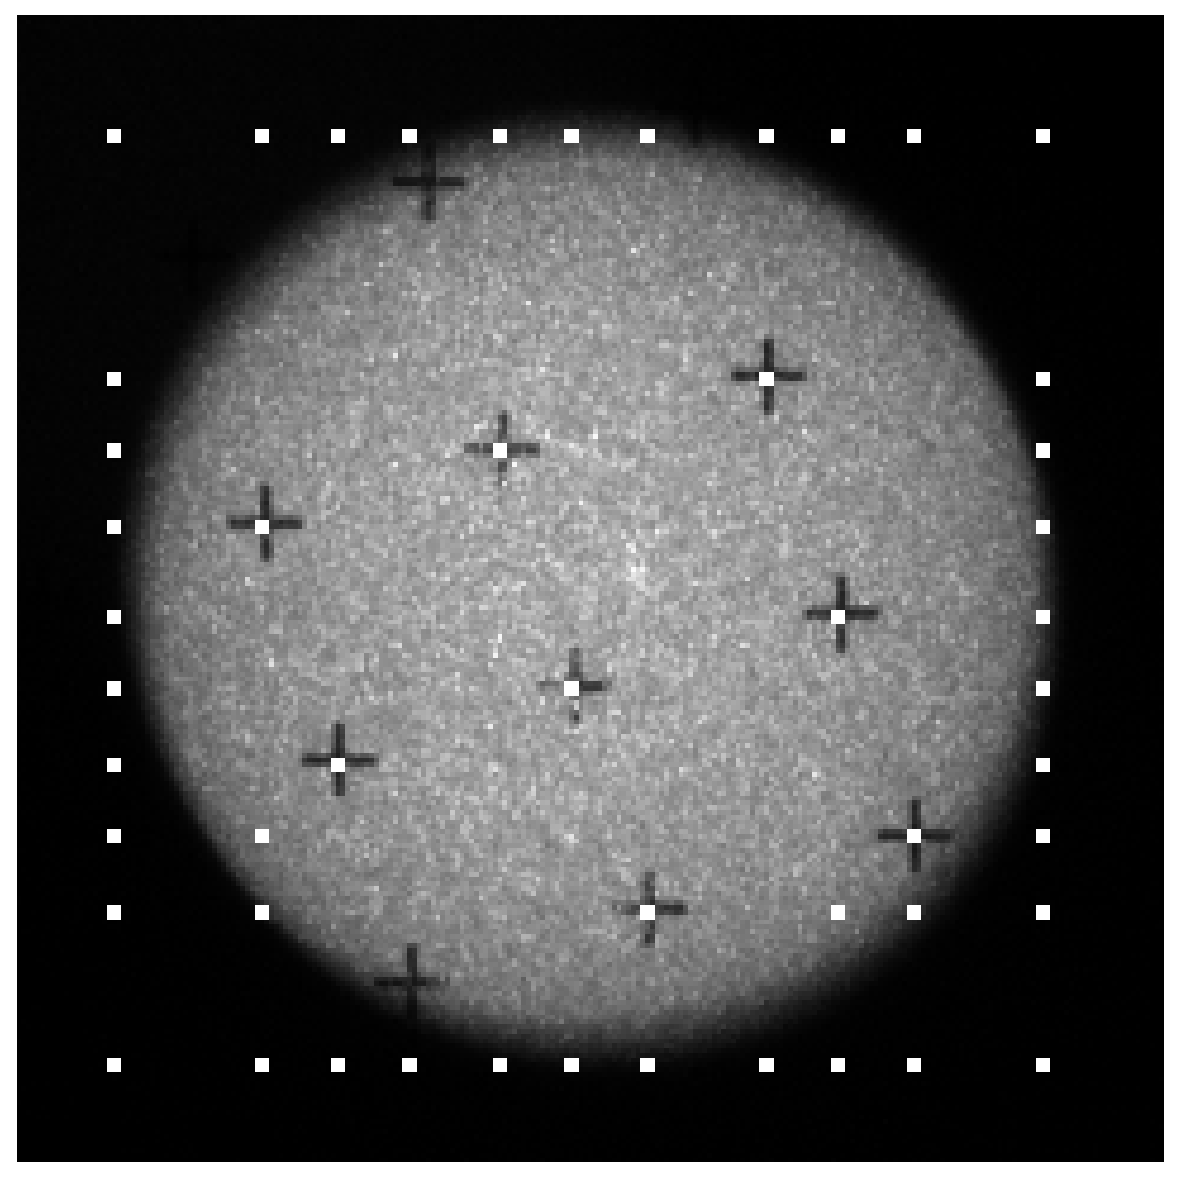
\includegraphics[width=.9\linewidth]{../plots_tables_images/dimenough.eps}
        }
        {
        \subcaption{Ruling out values above a certain threshold}
        }
    \end{subfloatrow}
}
{
\caption{}
\label{rulingout}
}
\end{figure}


Next, for the remaining candidates, we look at the 1D row and column sums to see if there are any obvious dips. \Cref{goodfid} is a fiducial candidate with obvious dips in the row/column arrays. \Cref{badfid} on the other hand, has a distinctive shape for 1D sums and does not have any obvious dips. Using another thresholding technique, we smooth the 1D sum and look for peaks in the difference of the smoothed 1D sum minus the 1D sum. If there are any pixels above this secondary 1D sum threshold, then the fiducial candidate is considered a bona-fide fiducial.  

\begin{figure}[!ht]
\ffigbox{
    \begin{subfloatrow}
        \ffigbox[\FBwidth]% Width of subfloat
        {
        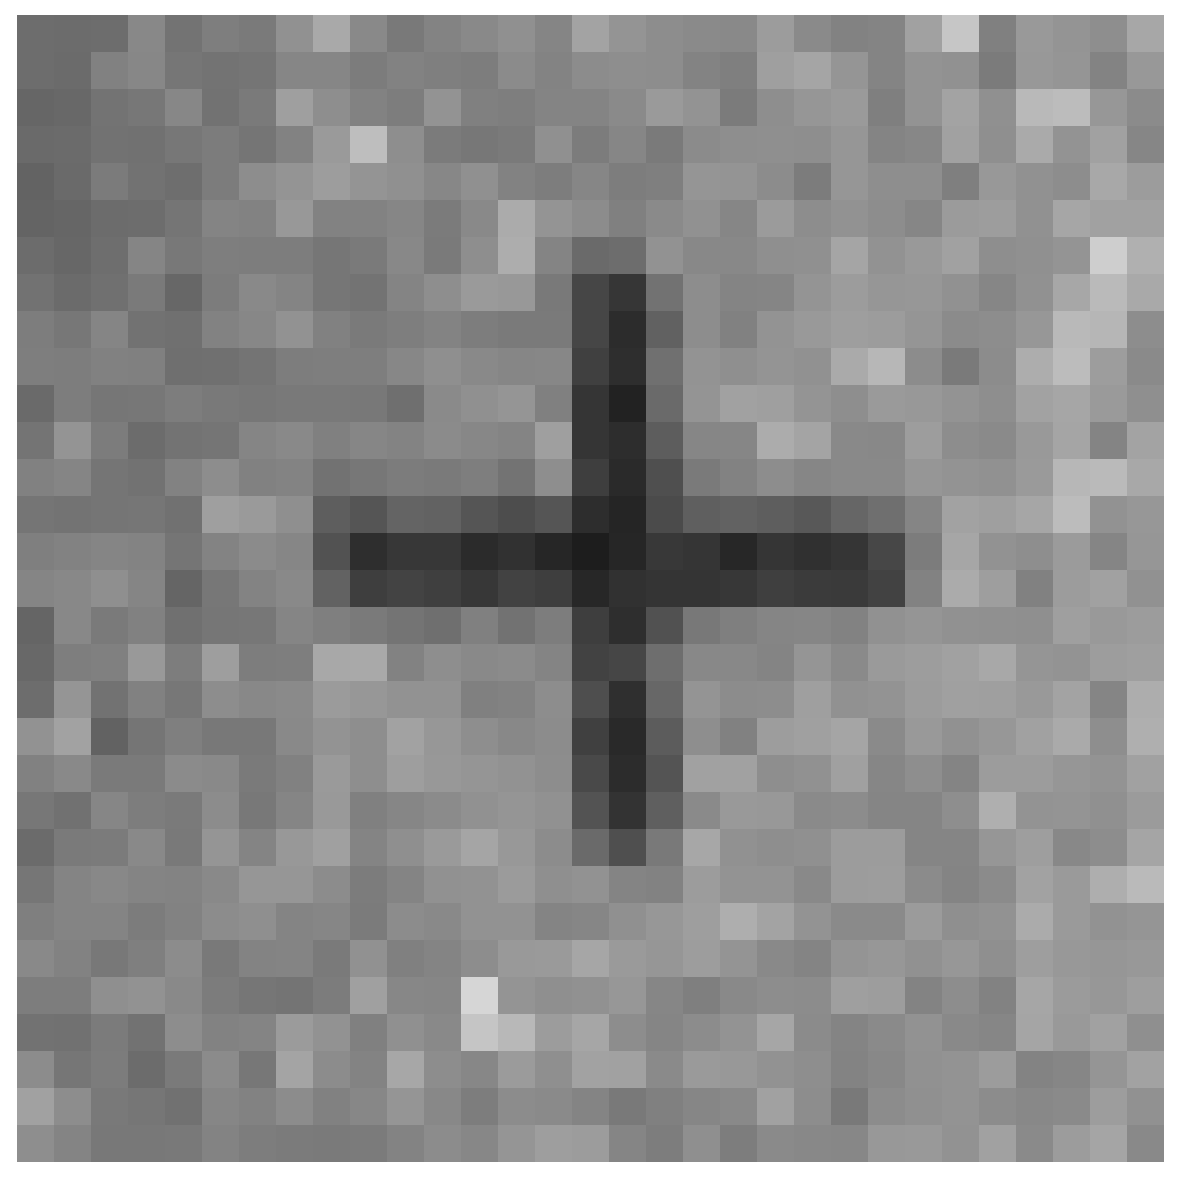
\includegraphics[width=.9\linewidth]{../plots_tables_images/fidcand_test.eps}
        }
        {
        \subcaption{Cropped region of a fiducial candidate}
        }
    \end{subfloatrow}
    \begin{subfloatrow}
        \ffigbox[\FBwidth]% Width of subfloat
        {
        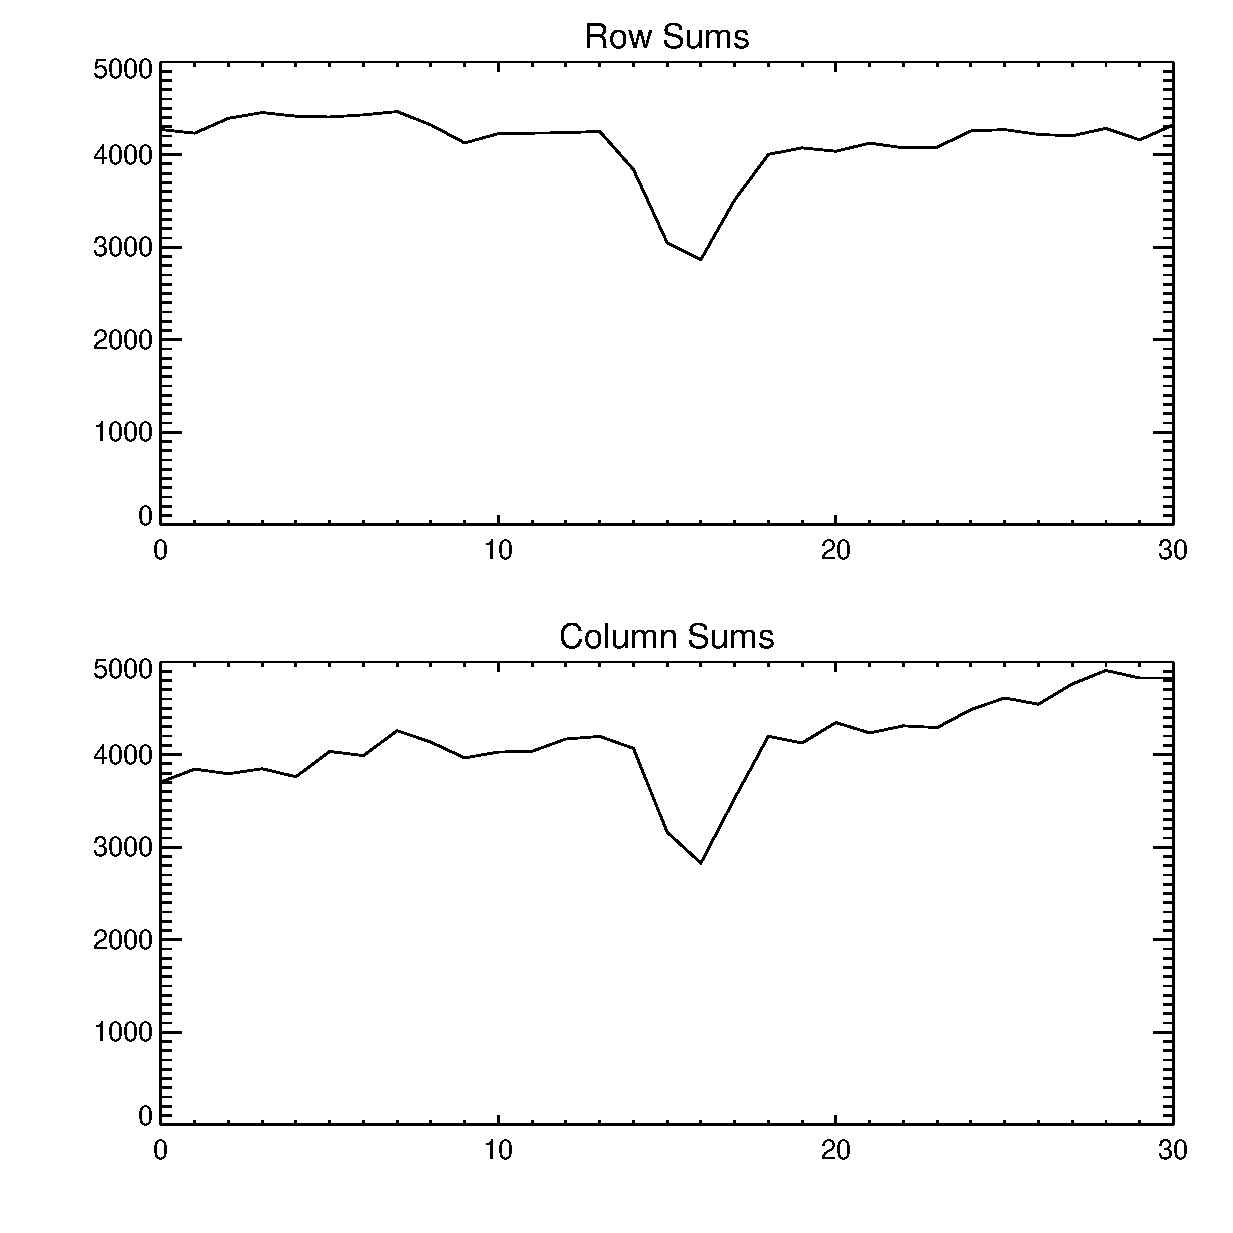
\includegraphics[width=.9\linewidth]{../plots_tables_images/fidcand_sums.eps}
        }
        {
        \subcaption{1D sums of cropped region}
        }
    \end{subfloatrow}
}
{
\caption{}
\label{goodfid}
}
\end{figure}

\begin{figure}[!ht]
\ffigbox{
    \begin{subfloatrow}
        \ffigbox[\FBwidth]% Width of subfloat
        {
        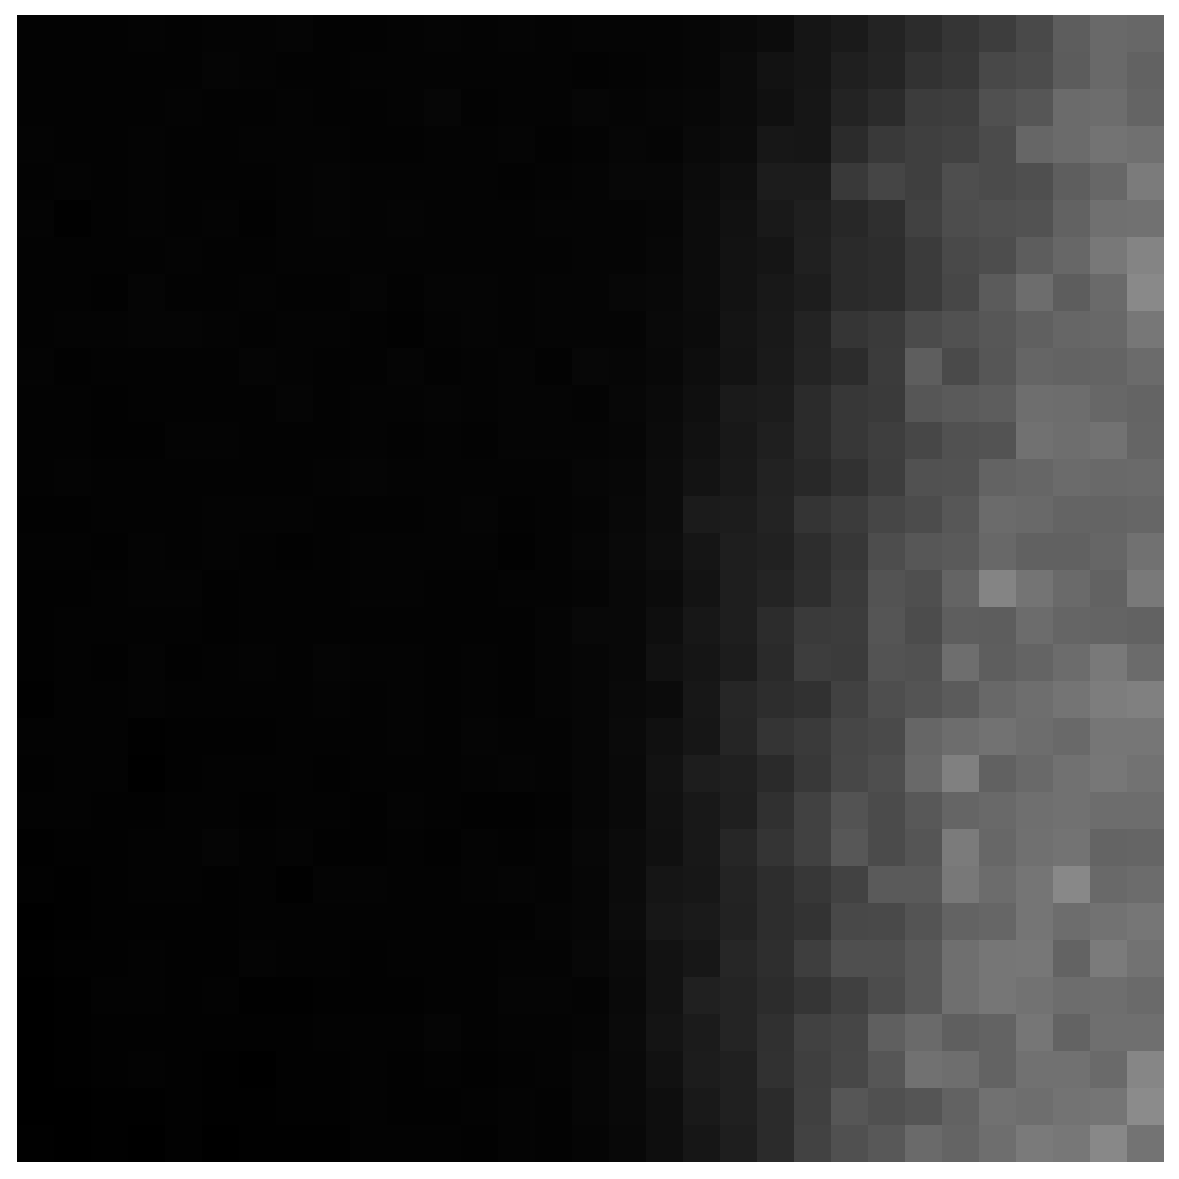
\includegraphics[width=.9\linewidth]{../plots_tables_images/badfid.eps}
        }
        {
        \subcaption{Cropped region of a fidcuail candidate}
        }
    \end{subfloatrow}
    \begin{subfloatrow}
        \ffigbox[\FBwidth]% Width of subfloat
        {
        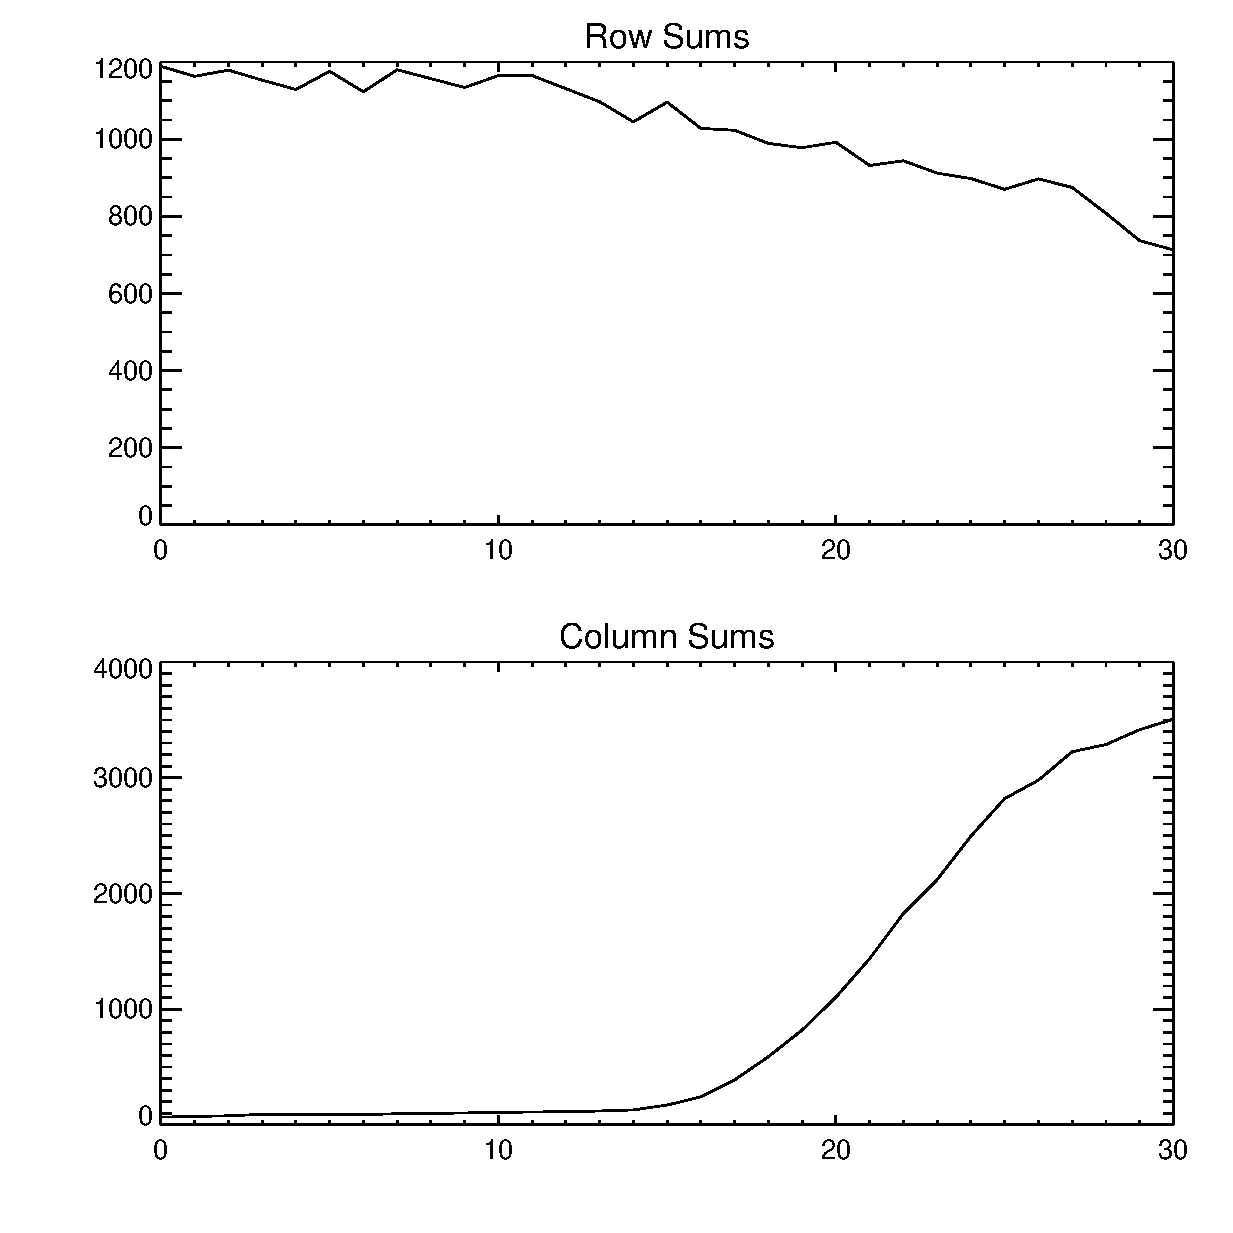
\includegraphics[width=.9\linewidth]{../plots_tables_images/fidcand_sums_falsepos.eps}
        }
        {
        \subcaption{1D sums of cropped region}
        }
    \end{subfloatrow}
}
{
\caption{}
\label{badfid}
}
\end{figure}
% subsection ruling_out_false_fiducial (end)

\subsection{Sub-pixel Fiducial Positions} % (fold)
\label{sub:sub_pixel_fiducial_positions}

Now that we have a column/row position of a fiducial, we look to find a sub-pixel location of the fiducial. Now, this technique has proven to be more efficient in past iterations of the program and is still under construction.\\
\indent In earlier versions of the program, we used a 2D convolution filter with a kernel that looks like a fiducial. Areas on the image that look like fiducials have high correlation values and thus peak in the 2D convolved array. Once we had computed the local maxima (which gave us rough fiducial positions), we used 2 1D parabolic fitting procedures to the peak of the local maxima. The location where the two parabolas intersect (since they're perpendicular to each other) is the sub-pixel parabolic fit for the fiducial position.\\
\indent In this version of the code, we don't have any natural peaks in the 2D image so we have to look for peaks elsewhere. Thankfully, we have peaks in the 1D sums. Instead of using a parabolic fit to the 2D convolution of the image, we fit a parabola to the peak of the 1D sum. Same deal, we look where the two parabolas intersect. I'm honestly not sure if I can do this but for now this is how we're doing it.\\
\indent After thresholding the peak of the fiducial candidate's 1D sum, we end up with \cref{fiddone}.

\begin{figure}[!ht]
    \centering
    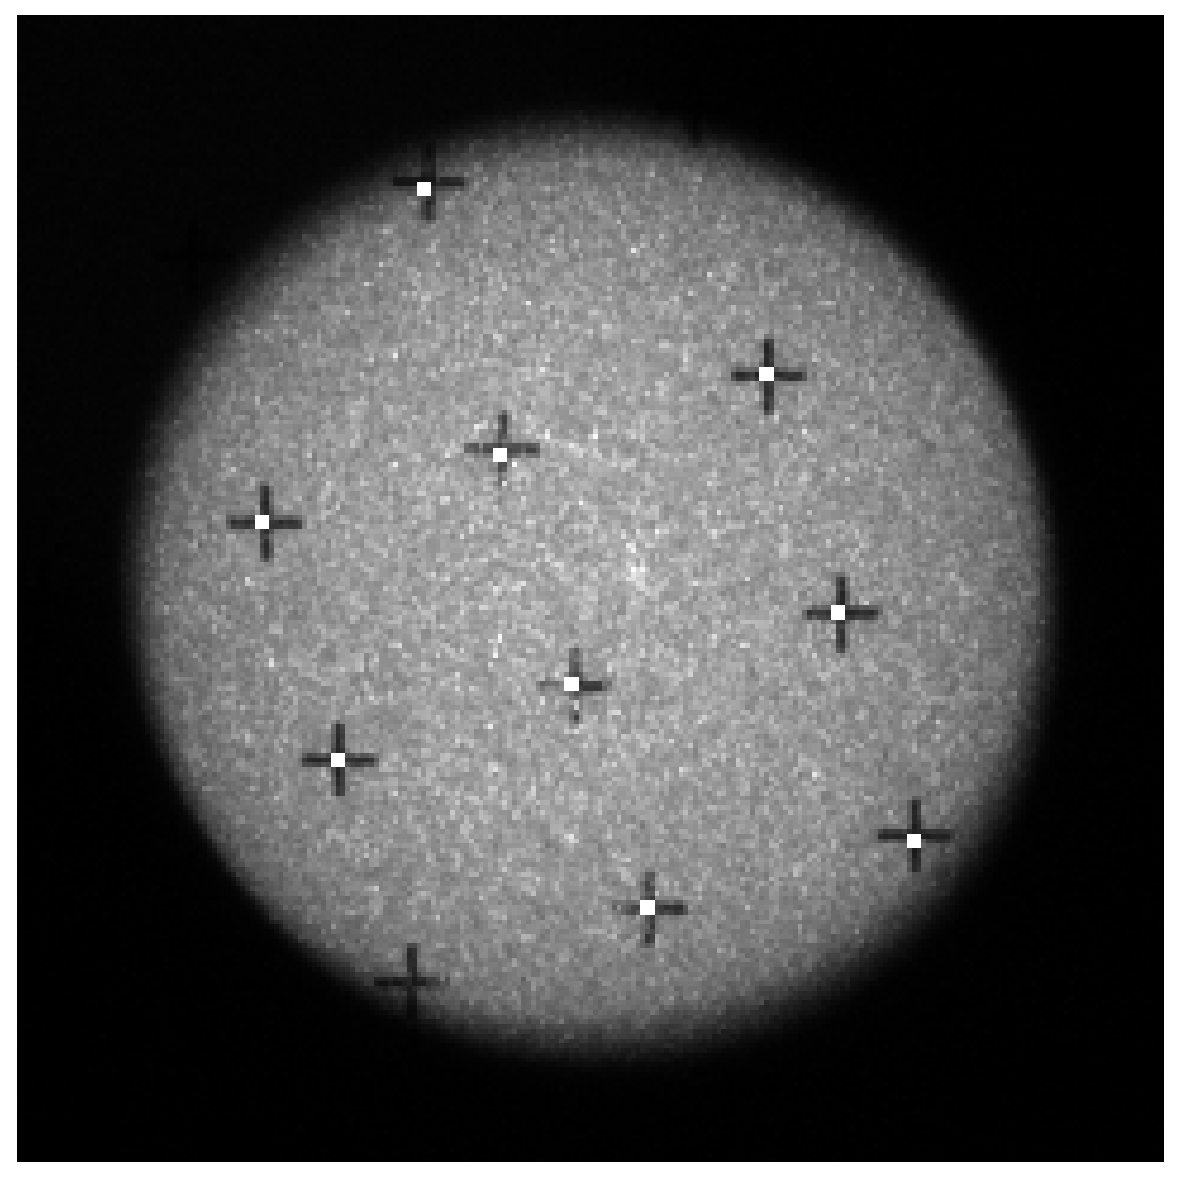
\includegraphics[width=.9\textwidth]{../plots_tables_images/fiddone.eps}
    \caption{Final set of fiducials}
    \label{fiddone}
\end{figure}

% subsection sub_pixel_fiducial_positions (end)
% section finding_ficuials (end)

\section{Final Words} % (fold)
\label{sec:final_words}

\Cref{structtable} is an example of how the final data structure is kept. Since the number of fiducials cannot be predetermined and I don't know how to append structure elements within a nested structure, the fiducial positions are kept in a separate pointer structure which takes the form of \cref{fidtable}. The structure of the \hl{\texttt{FIDARR}} array is shown in \cref{fidposarr}. 

\begin{deluxetable}{clll}
    \tablecaption{Final data structure of solar region}
    \tablecolumns{4}
    \tabletypesize{\scriptsize}
    \tablewidth{0pt}
    \tablehead{ 
      \colhead{Name} %
    & \colhead{Type} %
    & \colhead{Value} %
    & \colhead{Notes}
    }
    \startdata
    XPOS
    & FLOAT
    & 875.802
    & Rough calculation using a simple masking method\\
    %
    YPOS
    & FLOAT
    & 544.078
    & ''\\
    %
    REG
    & INT
    & 1
    & Region ID \#: 1 is 100\%, 2 is 50\%, 3 is 25\%\\
    %
    THRESH
    & FLOAT
    & 106.000
    & Threshold calculated from sorting array and taking derivatives.\\ & & & Used in both finding rough X-Y center as well as the\\ & & & threshold for limb-fitting.\\
    %
    PARTIAL
    & FLOAT
    & 0.
    & Flag that determines if the solar region is cut off on the edge or not.\\ & & & 0 means that it is not cut off \\
    %
    XSTRIPS
    & STRUCTURE
    & -> WHOLEXSTRIPS Array[5]
    & Strucutre containing the strips of whole solar data\\ & & & bound by a cropped region chosen by XPOS and YPOS\\
    %
    YSTRIPS
    & STRUCTURE
    & -> WHOLEYSTRIPS Array[5]
    & ''\\
    %
    LIMBXSTRIPS
    & STRUCTURE
    & -> LIMBXSTRIPS Array[5]
    & LIMBSTRIPS contains a pair of arrays, ENDPOINTS and \\ & & & STARTPOINTS that mark the limbs of each strip of data from \\ & & & X/YSTRIPS\\
    %
    LIMBYSTRIPS
    & STRUCTURE
    & -> LIMBYSTRIPS Array[5]
    & ''\\
    %
    LIMBXPOS
    & FLOAT
    & 898.586
    & Center calculated from LIMBXSTRIPS\\
    %
    LIMBYPOS
    & FLOAT
    & 541.795
    & ''\\
    %
    NPIX
    & FLOAT
    & 26680.0
    & Number of pixels above threshold. Used to determine if the sun\\
    & & &was a partial, deprecated.
    \enddata
\label{structtable}
\end{deluxetable}

\begin{deluxetable}{clll}
    \tablecaption{Structure of pointer containing fiducial positions}
    \tablecolumns{4}
    \tabletypesize{\scriptsize}
    \tablewidth{0pt}
    \tablehead{ 
      \colhead{Name} %
    & \colhead{Type} %
    & \colhead{Value} %
    & \colhead{Notes}
    }
    \startdata
    REG
    & INT
    & 1
    & Region ID \#: 1 is 100\%, 2 is 50\%, 3 is 25\%\\
    %
    FIDARR
    & STRUCT
    & -> FIDPOS Array[11]
    & Structure containing the fiducial positions and sub-pixel positions
    \enddata
\label{fidtable}
\end{deluxetable}


\begin{deluxetable}{clll}
    \tablecaption{Structure of \hl{\texttt{FIDARR}} structure}
    \tablecolumns{4}
    \tabletypesize{\scriptsize}
    \tablewidth{0pt}
    \tablehead{ 
      \colhead{Name} %
    & \colhead{Type} %
    & \colhead{Value} %
    & \colhead{Notes}
    }
    \startdata
    X
    & FLOAT
    & 51.0000
    & X position found through first set of 1D sums\\
    %
    Y
    & FLOAT
    & 133.000
    & ''\\
    %
    SUBX
    & FLOAT
    & 51.8438
    & X position found with parabolic peak-fitting of second 1D sum\\
    %
    SUBY
    & FLOAT
    & 134.291
    & ''
    \enddata
\label{fidposarr}
\end{deluxetable}

% section final_words (end)


\end{document}
